% --------------------------------------------------------------
% This is all preamble stuff that you don't have to worry about.
% Head down to where it says "Start here"
% --------------------------------------------------------------

\documentclass[11pt]{scrartcl}

\usepackage[margin=2cm]{geometry}
\usepackage[protrusion=true,expansion=true]{microtype}
\usepackage[pdftex]{graphicx}
\usepackage{url}
\usepackage{csquotes}
\usepackage{cleveref}
\usepackage{amsmath,amsthm,amssymb,nicefrac}
\usepackage{graphicx}
\usepackage{algorithm, algorithmic}
\usepackage{multirow}


%%% Custom sectioning
%\usepackage{sectsty}
%\allsectionsfont{\normalfont\scshape\textbf}

%%%% Raccourcis pour les caract�res doubles

\def\NN{{\mathbb N}}    %naturels
\def\ZZ{{\mathbb Z}}     %entiers relatifs
\def\RR{{\mathbb R}}    %r�els
\def\QQ{{\mathbb Q}}    %r�els
\def\CC{{\mathbb C}}    %complexes
\def\HH{{\mathbb H}}    %quaternions / espace hyperbolique
\def\PP{{\mathbb P}}     %espace projectif / probabilité
\def\KK{{\mathbb K}}     %corps quelconques
\def\BB{{\mathbb B}} 
\def\EE{{\mathbb E}}    % espérance
\def\11{{\mathbf 1}}    % indicatrice

%%%% Raccourcis pour les caract�res gras math�matiques
\def\bA{{\mathbf A}}  \def\bG{{\mathbf G}} \def\bM{{\mathbf M}} \def\bS{{\mathbf S}} \def\bB{{\mathbf B}}  \def\bH{{\mathbf H}} \def\bN{{\mathbf N}} \def\bT{{\mathbf T}} \def\bC{{\mathbf C}}  \def\bI{{\mathbf I}} \def\bO{{\mathbf O}} \def\bU{{\mathbf U}} \def\bD{{\mathbf D}}  \def\bJ{{\mathbf J}} \def\bP{{\mathbf P}} \def\bV{{\mathbf V}} \def\bE{{\mathbf E}}  \def\bK{{\mathbf K}} \def\bQ{{\mathbf Q}} \def\bW{{\mathbf W}} \def\bF{{\mathbf F}}  \def\bL{{\mathbf L}} \def\bR{{\mathbf R}} \def\bX{{\mathbf X}} \def\bY{{\mathbf Y}}  \def\bZ{{\mathbf Z}} \def\b1{{\mathbf 1}}


%%%%%%raccourcis lettres calligraphi�es
\def\cA{{\mathcal A}}  \def\cG{{\mathcal G}} \def\cM{{\mathcal M}} \def\cS{{\mathcal S}} \def\cB{{\mathcal B}}  \def\cH{{\mathcal H}} \def\cN{{\mathcal N}} \def\cT{{\mathcal T}} \def\cC{{\mathcal C}}  \def\cI{{\mathcal I}} \def\cO{{\mathcal O}} \def\cU{{\mathcal U}} \def\cD{{\mathcal D}}  \def\cJ{{\mathcal J}} \def\cP{{\mathcal P}} \def\cV{{\mathcal V}} \def\cE{{\mathcal E}}  \def\cK{{\mathcal K}} \def\cQ{{\mathcal Q}} \def\cW{{\mathcal W}} \def\cF{{\mathcal F}}  \def\cL{{\mathcal L}} \def\cR{{\mathcal R}} \def\cX{{\mathcal X}} \def\cY{{\mathcal Y}}  \def\cZ{{\mathcal Z}}

%%%%%%raccourcis lettres gothiques

\def\mfA{{\mathfrak A}} \def\mfA{{\mathfrak P}} \def\mfS{{\mathfrak S}}\def\mfZ{{\mathfrak Z}} \def\mfM{{\mathfrak M}} \def\mfQ{{\mathfrak Q}} \def\mfE{{\mathfrak E}} \def\mfL{{\mathfrak L}} \def\mfW{{\mathfrak W}} \def\mfR{{\mathfrak R}} \def\mfK{{\mathfrak K}} \def\mfX{{\mathfrak X}} \def\mfT{{\mathfrak T}} \def\mfJ{{\mathfrak J}} \def\mfC{{\mathfrak C}} \def\mfY{{\mathfrak Y}} \def\mfH{{\mathfrak H}} \def\mfV{{\mathfrak V}}\def\mfU{{\mathfrak U}}\def\mfG{{\mathfrak G}} \def\mfB{{\mathfrak B}} \def\mfI{{\mathfrak I}} \def\mfF{{\mathfrak F}} \def\mfN{{\mathfrak N}} \def\mfO{{\mathfrak O}} \def\mfD{{\mathfrak D}} 

\def\mfa{{\mathfrak a}} \def\mfp{{\mathfrak p}} \def\mfs{{\mathfrak s}}  \def\mfz{{\mathfrak z}} \def\mfm{{\mathfrak m}} \def\mfq{{\mathfrak q}}  \def\mfe{{\mathfrak e}} \def\mfl{{\mathfrak l}} \def\mfw{{\mathfrak w}} \def\mfr{{\mathfrak r}} \def\mfk{{\mathfrak k}} \def\mfx{{\mathfrak x}} \def\mft{{\mathfrak t}} \def\mfj{{\mathfrak j}} \def\mfc{{\mathfrak c}} \def\mfy{{\mathfrak y}} \def\mfh{{\mathfrak h}} \def\mfv{{\mathfrak v}} \def\mfu{{\mathfrak u}} \def\mfg{{\mathfrak g}} \def\mfb{{\mathfrak b}} \def\mfi{{\mathfrak i}} \def\mff{{\mathfrak f}} \def\mfn{{\mathfrak n}} \def\mfo{{\mathfrak o}} \def\mfd{{\mathfrak d}}

%%%%%%definition d applications
    
\newcommand{\deffunction}[5]{
{#1}:
\left|
  \begin{array}{rcl}
    {#2} & \longrightarrow & {#3} \\
    {#4} & \longmapsto & {#5} \\
  \end{array}
\right.
}

%%%%%%operateurs
\newcommand\MixMatch{\operatorname{MixMatch}}
\newcommand\Mixup{\operatorname{Mixup}}
\newcommand\BoxMix{\operatorname{BoxMix}}
\newcommand{\BBoxes}[1]{\operatorname{BBoxes}\left({#1}\right)}
\newcommand{\Mult}{\operatorname{Mult}}



\begin{document}

% --------------------------------------------------------------
%                         Start here
% --------------------------------------------------------------

%%% Maketitle metadata
\newcommand{\horrule}[1]{\rule{\linewidth}{#1}} 	% Horizontal rule

\title{
		\vspace{-0.5in}
%		\usefont{OT1}{bch}{b}{n}
		\horrule{0.5pt} \\[0.4cm]
		\Large Emulating Satellite Tangential Scale Distortion \\
		\horrule{2pt} \\
}
\date{}


\maketitle


% --------------------------------------------------------------
%     You don't have to mess with anything below this line.
% --------------------------------------------------------------


Remote sensing systems, provide an instantaneous \enquote{snapshot} view of the Earth from directly overhead. Each detector essentially takes a \enquote{snapshot} of each ground resolution cell.

However, a distortion occurs due to the rotation of the scanning optics. As the sensor scans across each line, the distance from the sensor to the ground increases further away from the centre of the swath. Although the scanning mirror rotates at a constant speed, the relative motion of the sensor is faster (relative to the ground) and scans a larger area as it moves closer to the edges. This effect results in the compression of image features at points away from the nadir and is called \textbf{tangential scale distortion.}


\begin{figure}[h]\label{img:plane}
\centering
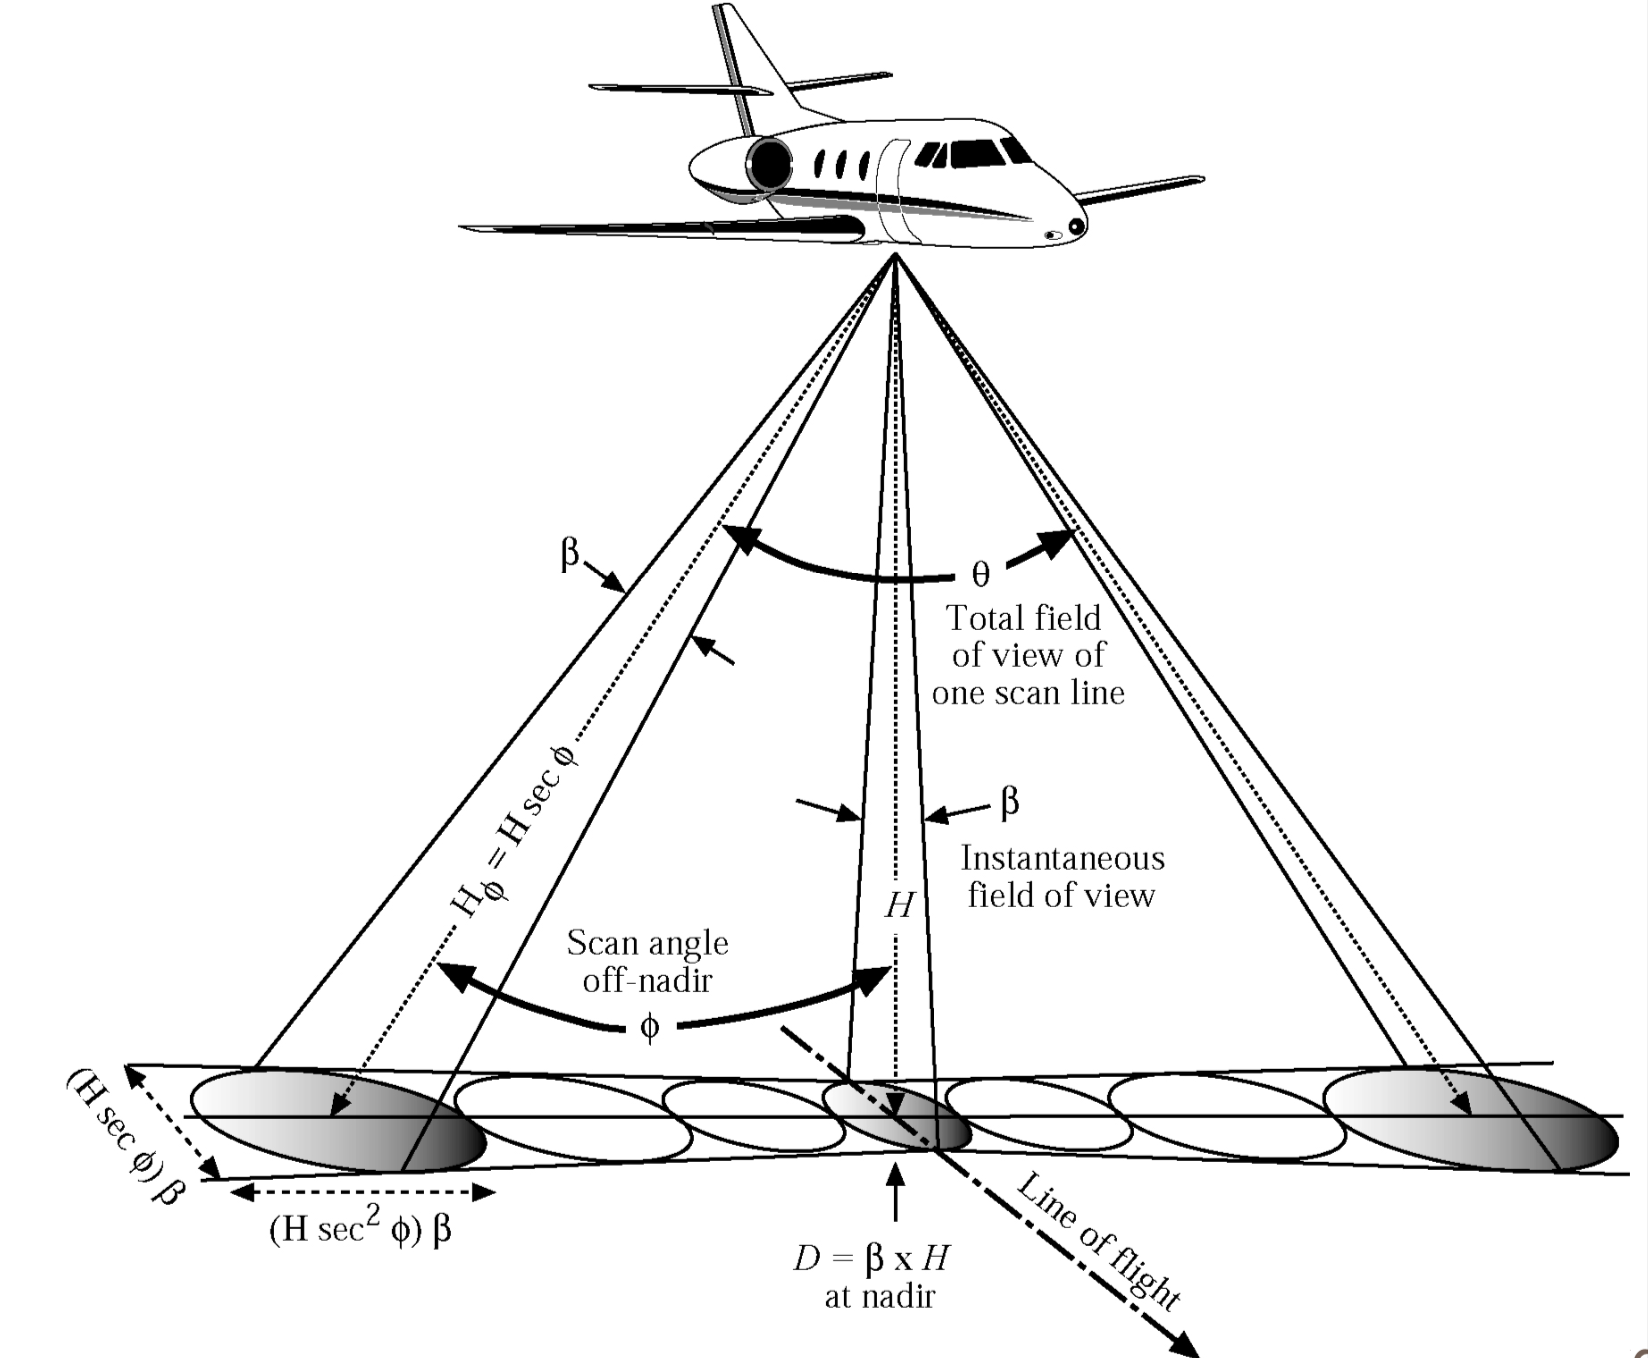
\includegraphics[width=0.6\textwidth]{img/plane_view.png}
\caption{The ground resolution cell size along a single across-track scan}
\end{figure}


To reflect this deformation when generating synthetic imagery samples, we propose to apply an unidimensional sigmoid application to coordinates along a virtual scanning line. Explicitely, let $\sigma_\lambda$ be :

$$
\deffunction{\sigma_\lambda}{\RR}{[0,1]}{x}{\frac{1}{1 + e^{-\lambda x}}}, \qquad \lambda >0
$$

Let now $\ell>0$ denote the image size along the deformation line and the center position $c = \frac{\ell}{2}$ corresponding to a virtual nadir. To reflect invariance at nadir and compression at edges, we apply along the swath line $[0, \ell]$ the application $x\in[0, \ell]\longmapsto\ell\sigma_\lambda(x - c)$.

In practice nearest method can be used for shifted pixels assignation and interpolation to cope with missing positions.

\begin{figure}[H]\label{img:deformation}
\centering
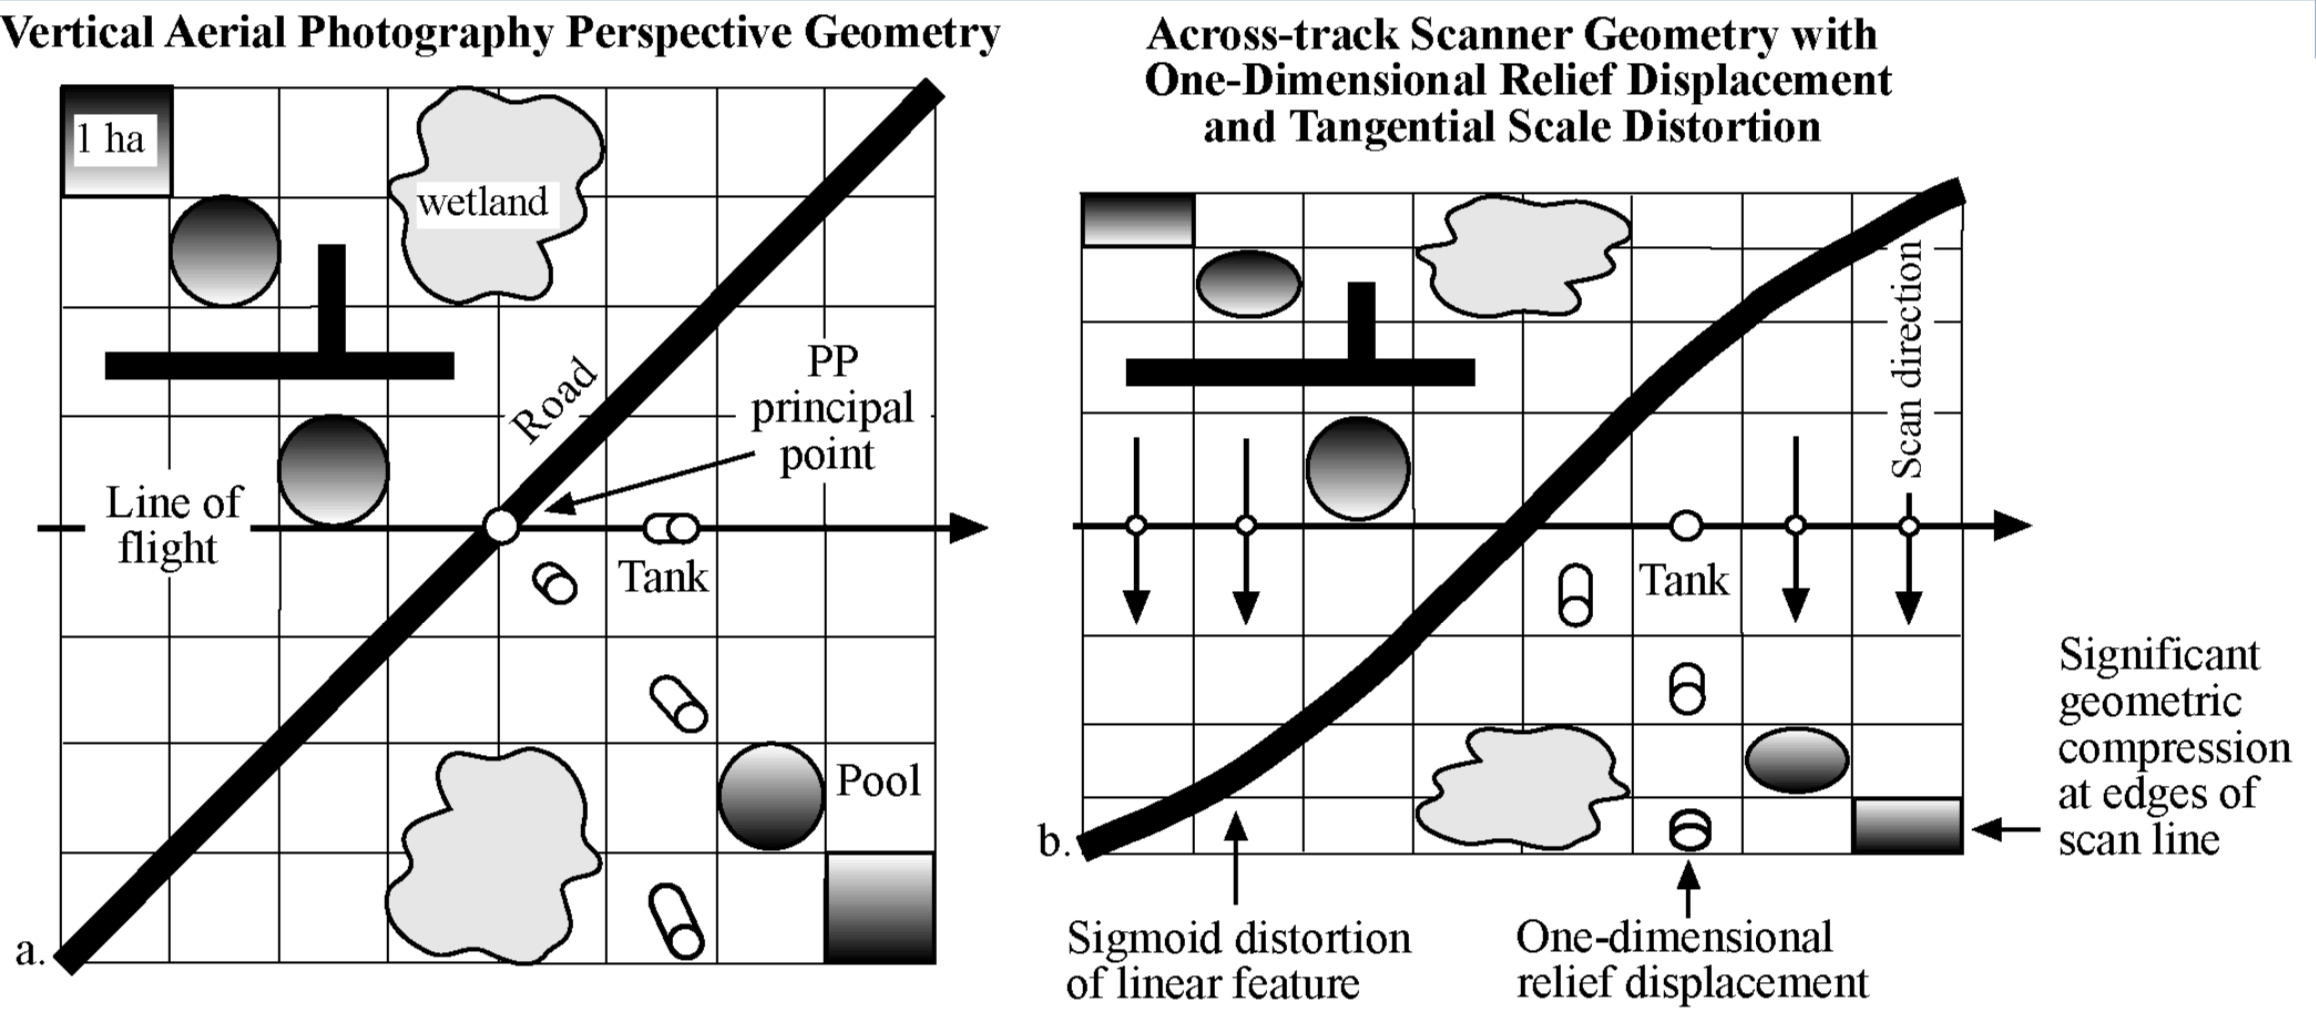
\includegraphics[width=0.7\textwidth]{img/sigmoid_deformation.png}
\caption{One-dimensional relief displacement is introduced in both directions away from nadir for each sweep of the across-track mirror. Linear features trending across the terrain are often recorded with s-shaped or sigmoid curvature characteristics due to tangential scale distortion and image compression.}
\end{figure}





Tangential scale distortion does not however expand image representation and only acts as a compression of the edges. Mathematically, it means that $x\mapsto\ell\sigma_\lambda(x - c)$ should be a contractive mapping. We find that setting $\lambda \leq \frac{4}{\ell}$ allows to satisfy this condition, proof is provided at the end.

This value sets an upper bound in the choice of $\lambda$ which can be used to model high-resolution satellites. For lower-resolution images generating larger deformation, lower values can be chosen.


\begin{figure}[H]\label{img:sigmoid}
\centering
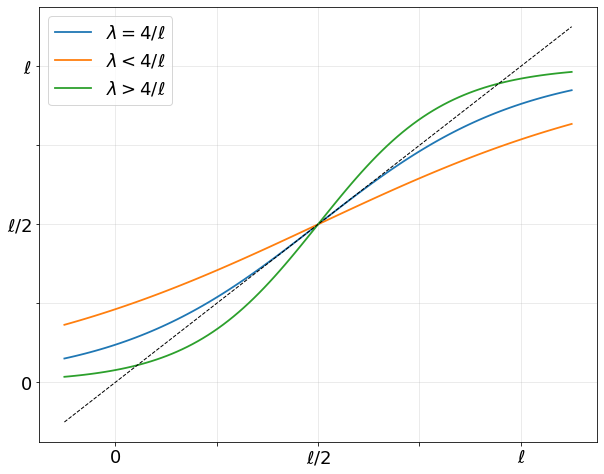
\includegraphics[width=0.5\textwidth]{img/sigmoids.png}
\caption{Plot of $\ell\sigma_\lambda(\cdot - c)$ for various choices of $\lambda$. In green, we observe the curve to grow faster than the identity, hence provoking interval expansion rather than compression.}
\end{figure}




\appendix

\begin{proof}\label{proof}

Let $\ell>0$ denote the image size along the deformation line and the center position $c = \frac{\ell}{2}$. In accordance with the previous notations, $\lambda$ must allow to satisfy :

\begin{align}
\forall x\leq c, \enspace \ell\sigma_\lambda(x - c)\geq x \label{eq:1}\\
\forall x\geq c, \enspace \ell\sigma_\lambda(x - c)\leq x \label{eq:2}
\end{align}


\begin{align}
\text{(\ref{eq:1})} &  \Rightarrow\forall x\in]0, c[\qquad x - c \geq \sigma_\lambda^{-1}\left(\frac{x}{\ell}\right) \\
& \Rightarrow\forall x\in]0, c[ \qquad \lambda \leq \sigma_{x - c}^{-1}\left(\frac{x}{\ell}\right)
\end{align}

where $\sigma_\lambda^{-1} = x\in]0,1[\longmapsto\frac{1}{\lambda}\log\left(\frac{x}{1 - x}\right)$.

Similarly,

\begin{align}
\text{(\ref{eq:2})}&  \Rightarrow\forall x\in]c, \ell[\qquad x - c \leq \sigma_\lambda^{-1}\left(\frac{x}{\ell}\right) \\
& \Rightarrow\forall x\in]c, \ell[ \qquad \lambda \leq \sigma_{x - c}^{-1}\left(\frac{x}{\ell}\right)
\end{align}


Hence $\forall x \in ]0, \ell[\smallsetminus\{c\}$ we have

$$
\lambda \leq \frac{1}{x-c}\log\left(\frac{\nicefrac{x}{\ell}}{1 - \nicefrac{x}{\ell}}\right) = \underbrace{\frac{1}{x - c}\log\left(\frac{x}{\ell - x}\right)}_{\psi_\ell(x)}
$$

$\psi_\ell$ decreases on $]0, c[$ and increases on $]c, \ell[$. It thus admits a lower bound in $c$, i.e.

$$
\underset{]0, \ell[\backslash\{c\}}{\lim\inf}\psi_\ell = \lim_{x\rightarrow c}\psi_\ell(x)
$$

To compute this limit, we observe that :

\begin{align*}
\log\left(\frac{x}{\ell - x}\right) & = \log(x) - \log(\ell - x) \\
& = \log\left(c + \left(x - c\right)\right) - \log\left(c - \left(x - c\right)\right) \\
& \underset{x \rightarrow c}{=}\frac{x - c}{c} + \frac{x - c}{c} + o\left(x - c\right) \\
& \underset{x \rightarrow c}{=} \frac{4}{\ell}\left(x - c\right) + o\left(x - c\right)
\end{align*}

Which entails :

$$
\psi_\ell(x)\underset{x \rightarrow c}{=}\frac{1}{x-c}\left[\frac{4}{\ell}\left(x - c\right) + o\left(x - c\right)\right] \underset{x \rightarrow c}{=}\frac{4}{\ell} + o(1)\Rightarrow \lim_{x\rightarrow c}\psi_\ell(x) = \frac{4}{\ell}
$$

Reversely, we verify that choosing $\lambda \leq \frac{4}{\ell}$ allows to verify (\ref{eq:1}) and (\ref{eq:2}), hence making $x\mapsto\ell\sigma_\lambda(x-c)$ contractive.
\end{proof}

\end{document}
